\documentclass[14pt]{extbook}
\usepackage{multicol, enumerate, enumitem, hyperref, color, soul, setspace, parskip, fancyhdr} %General Packages
\usepackage{amssymb, amsthm, amsmath, latexsym, units, mathtools} %Math Packages
\everymath{\displaystyle} %All math in Display Style
% Packages with additional options
\usepackage[headsep=0.5cm,headheight=12pt, left=1 in,right= 1 in,top= 1 in,bottom= 1 in]{geometry}
\usepackage[usenames,dvipsnames]{xcolor}
\usepackage{dashrule}  % Package to use the command below to create lines between items
\newcommand{\litem}[1]{\item#1\hspace*{-1cm}\rule{\textwidth}{0.4pt}}
\pagestyle{fancy}
\lhead{Makeup Progress Quiz 3}
\chead{}
\rhead{Version B}
\lfoot{1648-1753}
\cfoot{}
\rfoot{Summer C 2021}
\begin{document}

\begin{enumerate}
\litem{
Solve the equation below. Then, choose the interval that contains the solution.\[ -5(-12x -6) = -15(14x -4) \]\begin{enumerate}[label=\Alph*.]
\item \( x \in [-0.38, -0.32] \)
\item \( x \in [0.5, 1.22] \)
\item \( x \in [0.25, 0.44] \)
\item \( x \in [-0.08, 0.22] \)
\item \( \text{There are no real solutions.} \)

\end{enumerate} }
\litem{
Find the equation of the line described below. Write the linear equation in the form $ y=mx+b $ and choose the intervals that contain $m$ and $b$.\[ \text{Perpendicular to } 3 x - 7 y = 6 \text{ and passing through the point } (-4, -4). \]\begin{enumerate}[label=\Alph*.]
\item \( m \in [-2.6, -1.6] \hspace*{3mm} b \in [-18.33, -11.33] \)
\item \( m \in [1.4, 3.4] \hspace*{3mm} b \in [4.33, 13.33] \)
\item \( m \in [-1.3, 0.6] \hspace*{3mm} b \in [-18.33, -11.33] \)
\item \( m \in [-2.6, -1.6] \hspace*{3mm} b \in [-3, 3] \)
\item \( m \in [-2.6, -1.6] \hspace*{3mm} b \in [9.33, 15.33] \)

\end{enumerate} }
\litem{
Find the equation of the line described below. Write the linear equation in the form $ y=mx+b $ and choose the intervals that contain $m$ and $b$.\[ \text{Parallel to } 5 x + 7 y = 11 \text{ and passing through the point } (-8, -5). \]\begin{enumerate}[label=\Alph*.]
\item \( m \in [0.26, 1.53] \hspace*{3mm} b \in [-1.3, 2.8] \)
\item \( m \in [-2.29, -0.89] \hspace*{3mm} b \in [-13.3, -9.8] \)
\item \( m \in [-0.83, -0.61] \hspace*{3mm} b \in [9.8, 10.9] \)
\item \( m \in [-0.83, -0.61] \hspace*{3mm} b \in [1.3, 3.8] \)
\item \( m \in [-0.83, -0.61] \hspace*{3mm} b \in [-13.3, -9.8] \)

\end{enumerate} }
\litem{
Write the equation of the line in the graph below in Standard Form $Ax+By=C$. Then, choose the intervals that contain $A, B, \text{ and } C$.
\begin{center}
    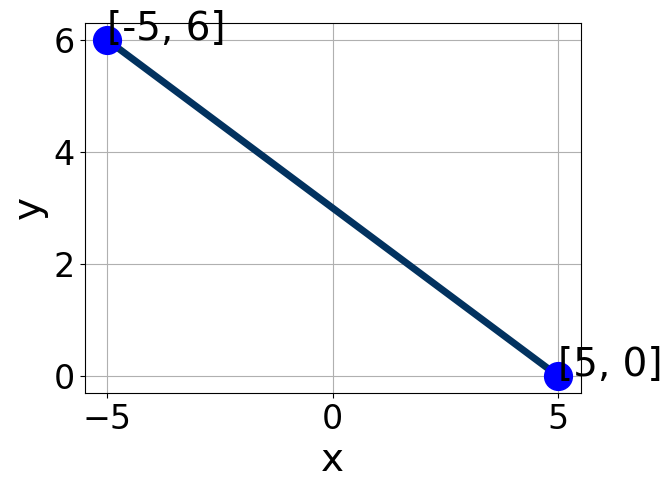
\includegraphics[width=0.5\textwidth]{../Figures/linearGraphToStandardCopyB.png}
\end{center}
\begin{enumerate}[label=\Alph*.]
\item \( A \in [1.1, 6.7], \hspace{3mm} B \in [4, 8], \text{ and } \hspace{3mm} C \in [14, 21] \)
\item \( A \in [0.4, 0.8], \hspace{3mm} B \in [1, 3], \text{ and } \hspace{3mm} C \in [3, 6] \)
\item \( A \in [1.1, 6.7], \hspace{3mm} B \in [-8, -4], \text{ and } \hspace{3mm} C \in [-16, -13] \)
\item \( A \in [-5.2, 0.2], \hspace{3mm} B \in [-8, -4], \text{ and } \hspace{3mm} C \in [-16, -13] \)
\item \( A \in [0.4, 0.8], \hspace{3mm} B \in [-4, 0], \text{ and } \hspace{3mm} C \in [-3, -2] \)

\end{enumerate} }
\litem{
Solve the linear equation below. Then, choose the interval that contains the solution.\[ \frac{7x -8}{5} - \frac{-4x -7}{3} = \frac{6x -9}{4} \]\begin{enumerate}[label=\Alph*.]
\item \( x \in [-0.5, 2.8] \)
\item \( x \in [-8.1, -5.8] \)
\item \( x \in [-1.1, 1.1] \)
\item \( x \in [-3.4, -1] \)
\item \( \text{There are no real solutions.} \)

\end{enumerate} }
\litem{
First, find the equation of the line containing the two points below. Then, write the equation in the form $ y=mx+b $ and choose the intervals that contain $m$ and $b$.\[ (-4, -6) \text{ and } (8, -11) \]\begin{enumerate}[label=\Alph*.]
\item \( m \in [-2.9, 0.3] \hspace*{3mm} b \in [-3.5, 0.2] \)
\item \( m \in [-2.9, 0.3] \hspace*{3mm} b \in [6.7, 8.3] \)
\item \( m \in [-0.4, 1] \hspace*{3mm} b \in [-17, -13.7] \)
\item \( m \in [-2.9, 0.3] \hspace*{3mm} b \in [-22.3, -17] \)
\item \( m \in [-2.9, 0.3] \hspace*{3mm} b \in [-8.4, -6.1] \)

\end{enumerate} }
\litem{
Write the equation of the line in the graph below in Standard Form $Ax+By=C$. Then, choose the intervals that contain $A, B, \text{ and } C$.
\begin{center}
    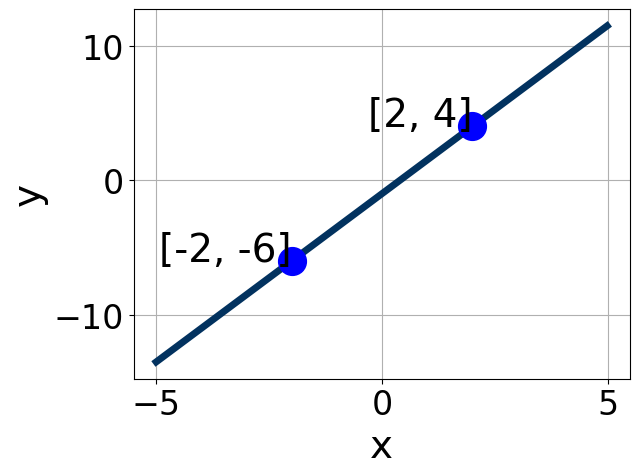
\includegraphics[width=0.5\textwidth]{../Figures/linearGraphToStandardB.png}
\end{center}
\begin{enumerate}[label=\Alph*.]
\item \( A \in [1.2, 7.5], \hspace{3mm} B \in [-2.09, -1.98], \text{ and } \hspace{3mm} C \in [1.77, 2.7] \)
\item \( A \in [-8.3, -4.3], \hspace{3mm} B \in [1.68, 2.11], \text{ and } \hspace{3mm} C \in [-2.34, -1.66] \)
\item \( A \in [-3.3, -2], \hspace{3mm} B \in [0.56, 1.64], \text{ and } \hspace{3mm} C \in [-1.47, 0.03] \)
\item \( A \in [1.2, 7.5], \hspace{3mm} B \in [1.68, 2.11], \text{ and } \hspace{3mm} C \in [-2.34, -1.66] \)
\item \( A \in [-3.3, -2], \hspace{3mm} B \in [-1.39, -0.82], \text{ and } \hspace{3mm} C \in [0.25, 1.12] \)

\end{enumerate} }
\litem{
Solve the equation below. Then, choose the interval that contains the solution.\[ -15(-9x -12) = -4(-18x -17) \]\begin{enumerate}[label=\Alph*.]
\item \( x \in [3.66, 4.21] \)
\item \( x \in [-4.56, -3.75] \)
\item \( x \in [-2.55, -1.28] \)
\item \( x \in [-1.65, 0.08] \)
\item \( \text{There are no real solutions.} \)

\end{enumerate} }
\litem{
First, find the equation of the line containing the two points below. Then, write the equation in the form $ y=mx+b $ and choose the intervals that contain $m$ and $b$.\[ (11, 2) \text{ and } (9, -11) \]\begin{enumerate}[label=\Alph*.]
\item \( m \in [4.5, 8.5] \hspace*{3mm} b \in [-74.5, -67.5] \)
\item \( m \in [-14.5, -4.5] \hspace*{3mm} b \in [46.5, 50.5] \)
\item \( m \in [4.5, 8.5] \hspace*{3mm} b \in [-15, -6] \)
\item \( m \in [4.5, 8.5] \hspace*{3mm} b \in [-20, -17] \)
\item \( m \in [4.5, 8.5] \hspace*{3mm} b \in [65.5, 71.5] \)

\end{enumerate} }
\litem{
Solve the linear equation below. Then, choose the interval that contains the solution.\[ \frac{-5x + 4}{7} - \frac{6x -3}{5} = \frac{-7x -4}{4} \]\begin{enumerate}[label=\Alph*.]
\item \( x \in [11.22, 16.22] \)
\item \( x \in [65.96, 67.96] \)
\item \( x \in [4.91, 8.91] \)
\item \( x \in [0.54, 1.54] \)
\item \( \text{There are no real solutions.} \)

\end{enumerate} }
\end{enumerate}

\end{document}